\documentclass{article}
\usepackage{tabularx}
\usepackage{amsmath}
\usepackage{graphicx}
\usepackage[margin=2cm]{geometry}
\usepackage{cite}
\usepackage[final]{hyperref}
\usepackage{listings}
\usepackage{here}
\hypersetup{
	colorlinks=true,
	linkcolor=blue,
	citecolor=blue,
	filecolor=magenta,
	urlcolor=blue         
}

\begin{document}

\title{TP03\\Noté}
\author{Robin Faury}
\date{25/01/2021}
\maketitle

\begin{abstract}
	\begin{figure}[H]
		\centering
		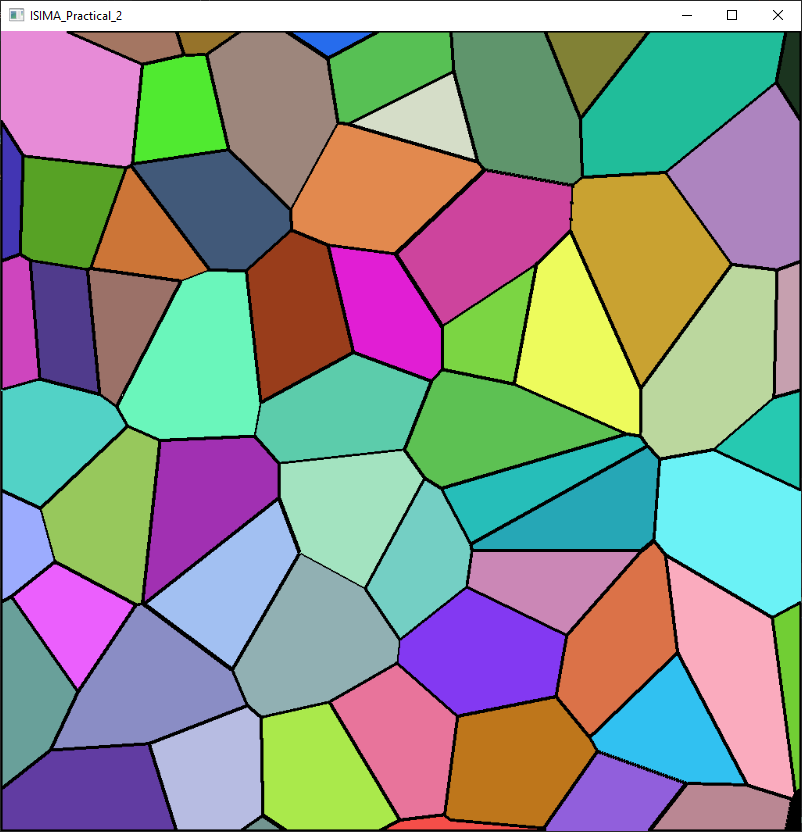
\includegraphics[scale=0.6]{images/intro.png}
		\caption{Segmentation d'une image}
	\end{figure}
\end{abstract}

\newpage
\section{Introduction}
\subsection{Clone du projet}
Les sources du projet sont accessibles à l'adresse suivante :
\begin{lstlisting}
	https://github.com/robinfaurypro/GPGPU_ISIMA_2020-2021.git
\end{lstlisting}
Le fichier CMakeLists se trouve dans le dossier Practical\_marked. Ouvrez une console et taper les commandes suivante :
\begin{lstlisting}
	git submodule update --init
	mkdir build
	cd build
	cmake -G "Visual Studio 15 Win64" ..
\end{lstlisting}
La dernière commande est à adapter si vous utilisez Visual Studio 2019 ou un système UNIX.
Si tout se passe correctement vous devriez voir une image représentant un diagramme de Voronoi.

\subsection{Modalité d'évaluation}
Le TP se déroule sur deux séances. C'est une illustration d'un cas réel que l'on peut rencontrer dans l'industrie. Le TP est donc volontairement très long et de difficulté croissante ce qui permet d'obtenir aisément la moyenne.\\
Le rendu de TP doit être fait avant le 08 mars 2021 sous la forme d'un fichier zip contenant les fichiers suivant :
\begin{itemize}
	\item Tous fichier sources ainsi que le CMakeLists si vous l'avez modifié. (Le dossier de build ne doit pas être rendu)
	\item Un compte rendu du TP où vous expliquerez les algorithmes que vous avez mis en place. Certain algorithme ne sont pas parallélisables et donc pas adaptable sur GPU. Il faudra aussi discuter de ces traitements dans le rapport.
\end{itemize}
Le rendu de TP compte pour 50\% de la note finale de la matière.

\section{Enoncé}
Il vous est proposé dans ce TP d'accélérer le traitement d'image effectuée par le logiciel. Actuellement, le programme lit une image d'entrée, détecte ses contours et remplit les cellules de couleur aléatoire. Tous les algorithmes de traitements d'images sont déjà développé en CPU. Vous devez donc utiliser les technologies GPGPU pour accélérer le traitement. Il est conseillé de suivre la méthode dites Assess, Parallelize, Optimize, Deploy. Les gains de vitesse devrons être exprimé en pourcentage.\\
Le but du traitement proposé ici est de faire une segmentation d'image. Pour cela, nous devons détecter les arêtes de l'image puis remplir les trous obtenus avec des couleurs aléatoire.

\subsection{Chargement de l'image}
Dans la fonction Initialization, vous trouverez le code pour charger une image depuis le dossier de ressource. Cette image est ouverte et stocké dans un vector de la structure content nommé image\_data\_color\_. Une texture GPU est aussi créé pour l'affichage du rendu final.
\begin{figure}[H]
	\centering
	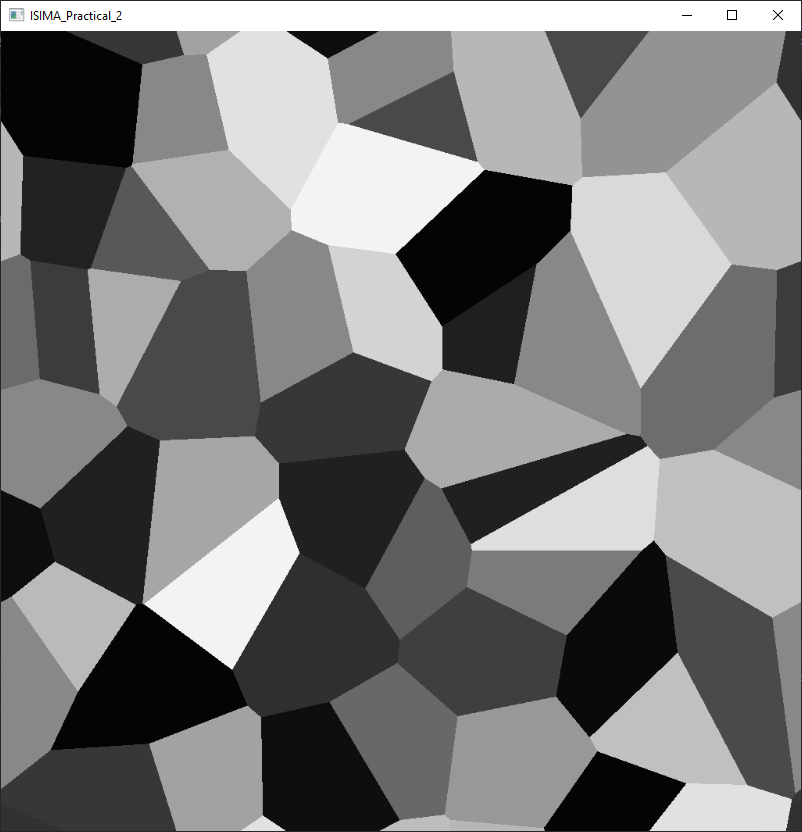
\includegraphics[scale=0.4]{images/input_image.png}
	\caption{Affichage de l'image d'entrée}
\end{figure}

\subsection{Passage en niveau de gris}
Les algorithmes qui suivent ont besoin de travailler sur des textures en niveau de gris. La fonction GrayscaleConversion sert donc à remplir le tableau image\_data\_grayscale\_. Le résultat visuel à la fin de cette étape doit être le même que pour la section précédente.

\subsection{Application d'un flou}
Souvent, les images d'entrée sont dites bruité ou présente de l'aliasing. Effectuer un flou aide à obtenir un résultat plus précis. Ici l'algorithme est un filtre moyenneur.
\begin{figure}[H]
	\centering
	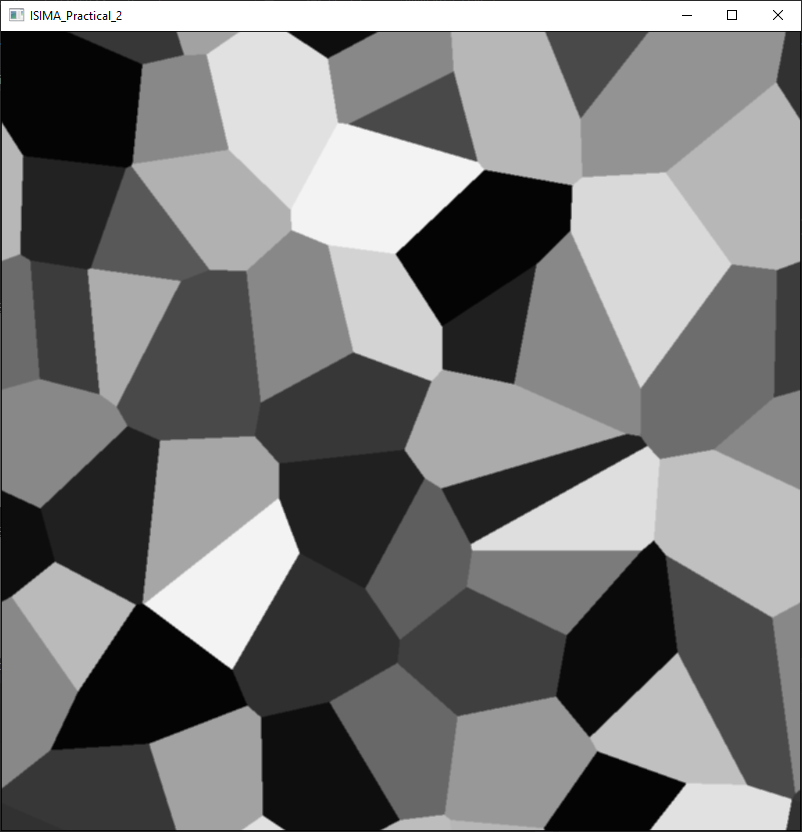
\includegraphics[scale=0.3]{images/blur.png}
	\caption{Image flouté}
\end{figure}

\subsection{Détection de contour}
La détection de contour s'effectue en utilisant un filtre de Sobel. Cela consiste à effectuer deux convolutions avec les deux noyaux de Sobel sur l'image pour obtenir un vecteur 2D décrivant le gradient de l'image.\\
Noyau de convolution de Sobel sur X = $\begin{pmatrix}-1&0&1\\ 
-2&0&2\\ 
-1&0&1\\ 
\end{pmatrix}$\\
Noyau de convolution de Sobel sur Y = $\begin{pmatrix}-1&-2&-1\\ 
0&0&0\\ 
1&2&1\\ 
\end{pmatrix}$\\
Le calcul de la norme de ce vecteur nous donne les contours de notre image.
\begin{figure}[H]
	\centering
	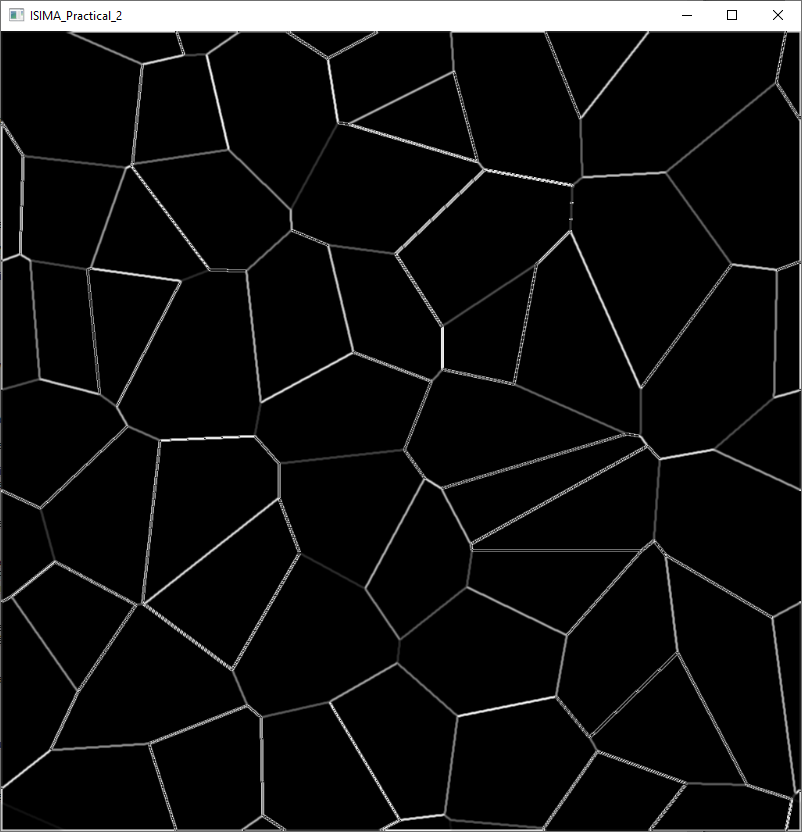
\includegraphics[scale=0.4]{images/sobel.png}
	\caption{Coutour de l'image}
\end{figure}

\subsection{Application d'un seuil}
Pour rendre plus lisible les contours, nous appliquons un seuil. Les valeurs situées au-dessus sont mises à la valeur maximale alors que les valeurs au-dessous sont mises à zéro.

\begin{figure}[H]
	\centering
	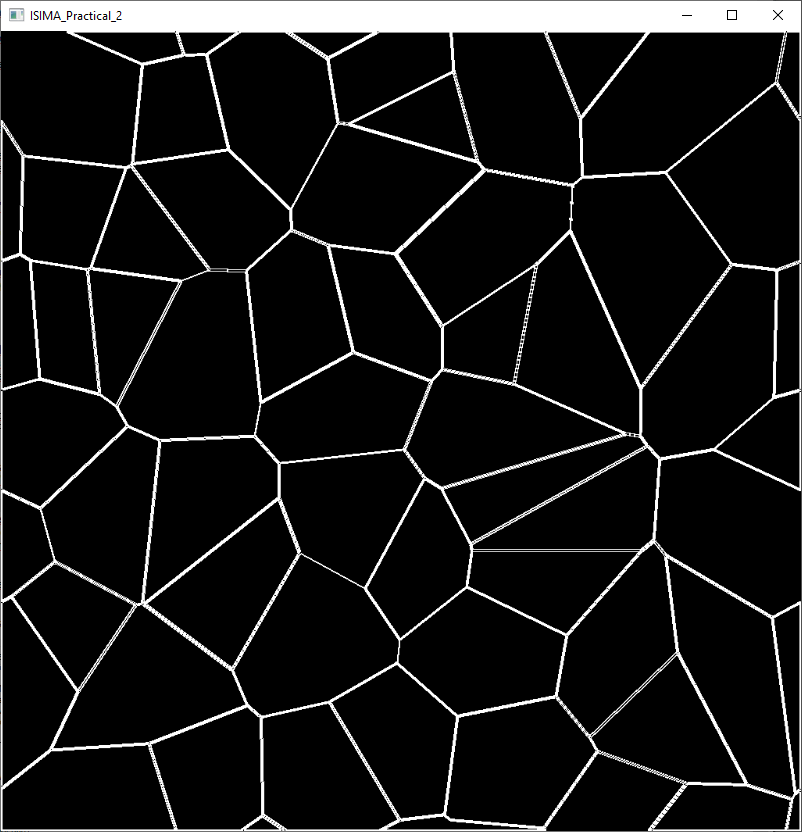
\includegraphics[scale=0.4]{images/level.png}
	\caption{Image binaire}
\end{figure}

\subsection{Ajout de seed}
L'algorithme que nous allons mettre en place consiste à placer les graines sur l'image et à les faire grandir. Si deux graines se rencontrent, elles fusionnent. On posera donc des graines de couleur de façon aléatoire sur toute l'image couleur sauf sur les contours.
\begin{figure}[H]
	\centering
	
\includegraphics[scale=0.4]{images/bruit.png}
	\caption{Image couleur avec les graines}
\end{figure}

\subsection{Remplissage des cellules}
Nous pouvons donc maintenant faire grossir nos cellules en utilisant l'algorithme de flood fill. Chaque graine va grossir et manger ces voisines dans chaque direction jusqu'à rencontrer un contour.
\begin{figure}[H]
	\centering
	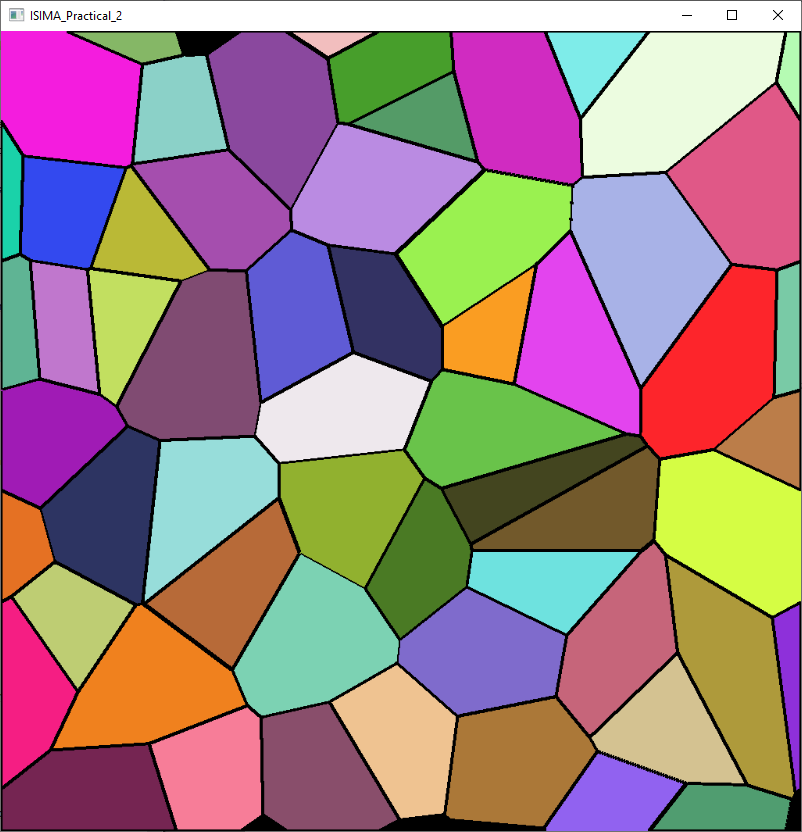
\includegraphics[scale=0.4]{images/flood_fill.png}
	\caption{Algorithme de remplissage}
\end{figure}

\subsection{Histogramme de l'image}
L'idée maintenant est de compter les cellules. Pour cela on fera l'histogramme de l'image et l'on comptera le nombre de couleur différente.

\section{Bonus}
On remarquera que le nombre de cellule n'est pas le même d'une frame à l'autre. Cela est dû à l'algorithme de détection de contour. En effet le filtre de Sobel détecte un contour sur les pixels avant la transition et après la transition. Nous avons donc potentiellement des cellules créées entre les bordures. Vous pouvez utiliser la dérivée seconde (filtre de Laplace) qui donne un seul contour par bordure.

\end{document}